% ------------------------------------------------------------------------------
% Este fichero es parte de la plantilla LaTeX para la realización de Proyectos
% Final de Grado, protegido bajo los términos de la licencia GFDL.
% Para más información, la licencia completa viene incluida en el
% fichero fdl-1.3.tex

% Copyright (C) 2012 SPI-FM. Universidad de Cádiz
% ------------------------------------------------------------------------------

\section{Introducción}
AssessMediaWiki es una aplicación web de código abierto que, al conectarse a una instalación MediaWiki, proporciona procedimientos de autoevaluación, hetero evaluación y evaluación entre iguales, a la vez que mantiene información sobre esas evaluaciones. Los supervisores pueden obtener informes que ayudan en la evaluación de los estudiantes.
\newline

Aunque hay un gran número de extensiones para el sistema MediaWiki, no hemos encontrado ninguna que permitiera evaluar contribuciones individuales a un wiki. La mayoría de las aproximaciones solo ofrecen formas de evaluar una versión en particular de un artículo (normalmente la más reciente), siendo ineficaces en este caso. Por ello, para evaluar la calidad de las contribuciones creamos AssessMediaWiki.
\newline

AssessMediaWiki implementa como base dos roles de usuario distintos: supervisores y estudiantes. Los estudiantes pueden elegir entre distintas opciones: evaluar una revisión, comprobar sus propias aportaciones evaluadas y verificar las evaluaciones ya enviadas. Por otro lado, los supervisores tienen un mayor número de opciones, como modificar los parámetros de los programas o vigilar las evaluaciones que los alumnos vayan haciendo.
\newline

\section{Características}
Las principales funcionalidades del sistema son:
\begin{itemize}
	\item Configurar ejercicios de evaluación.
	\item Evaluar ediciones al azar (dentro de las mas significativas).
	\item Generar CSV.
\end{itemize}

\section{Requisitos previos}
EL requisito principal es que debe haber un MediaWiki para que los alumnos trabajen sobre el.

\section{Uso del sistema}
Lo único necesario para poder usar el sistema es estar logeado en el MediaWiki existente, tras eso tan solo hay que seguir el manual de instalación y una vez se haya configurado el sistema podemos proceder a realizar pruebas del mismo, creando usuarios en el MediaWiki y realizando ediciones para posteriormente evaluarlas.\\

Si fuese necesario cualquier ayuda adicional, al final la sección de parámetros del sistema se encuentra un enlace a una sección de ayuda para el usuario, con información detallada de las opciones configurables del sistema con las que el docente deberá trabajar.

\begin{figure}[h]
	\centering
	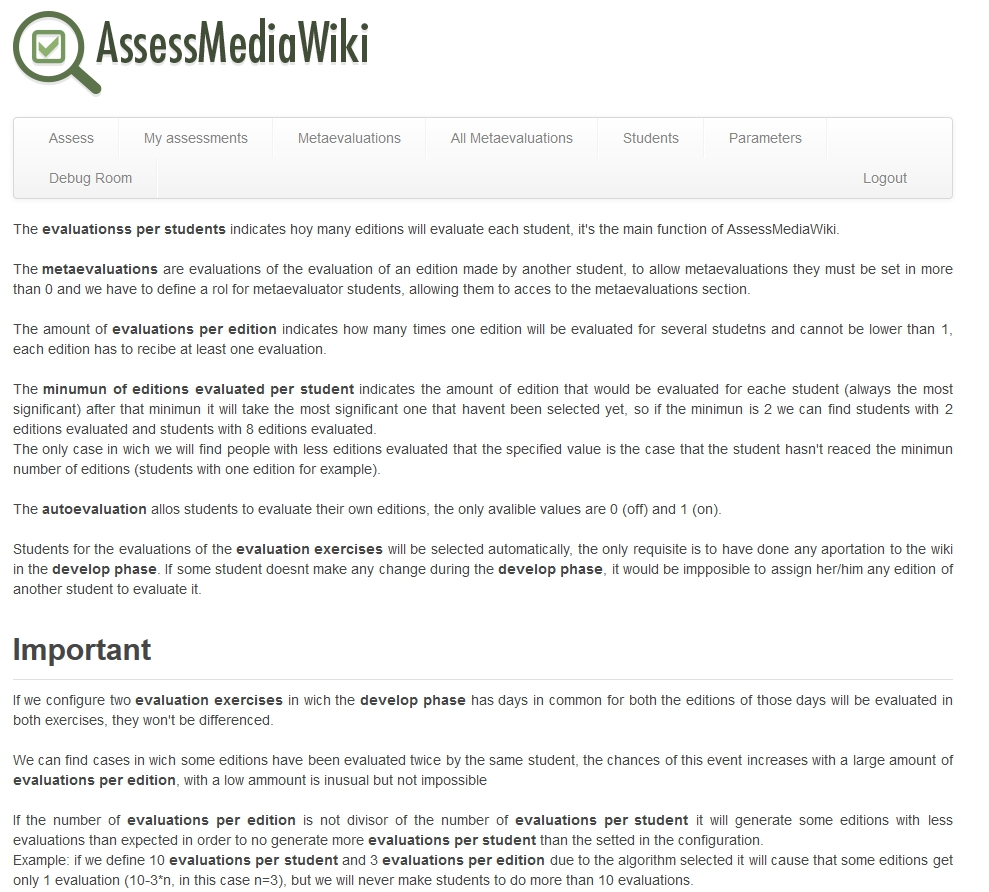
\includegraphics[width=0.9\textwidth]{sc_extra_help.jpg}
	\caption{Pantalla de ayuda extra.}
\end{figure}





